% Originally: content/week-02.tex, \section{Structured spaces} (Corsin Week 2, Monday)

\section{Structured spaces}
\label{sec:structured_spaces}

This semester, you will be introduced to certain structures that can be given to a set, which in
this context is also called a \newterm{space} \germanfor{Raum} and which we will denote by $X$:

\begin{itemize}
  \item \textbf{0. Topological spaces:} fourth semester.
  % German mirror deliberately omitted here: this bullet is a preview, and the first *formal*
  % introduction of the term is \cref{def:metric_space}, which carries the \germanterm pair.
  \item \textbf{1. Metric spaces} $(X,\ d : X \times X \to \mathbb{R}_{\geq 0})$
    \begin{itemize}
      \item Defines a \textbf{distance} between points.
      \item $X$ is \textbf{not} necessarily a vector space.
      \item Covered in \textit{Analysis}.
    \end{itemize}
  \item \textbf{2. Normed metric spaces} $(X,\ \|\cdot\| : X \to \mathbb{R}_{\geq 0})$
    \begin{itemize}
      \item Defines the \textbf{length} of a vector.
      \item Presupposes a linear structure: $X$ must be a \textbf{vector space}.
      \item Covered in \textit{Linalg / Analysis}.
    \end{itemize}
  \item \textbf{3. Inner product spaces} $(X,\ \langle\cdot,\cdot\rangle : X \times X \to \mathbb{R})$
    \begin{itemize}
      \item Defines \textbf{both} lengths \textbf{and} angles!
      \item Super important!
      \item Covered in \textit{Linalg} (and sometimes used in \textit{Analysis}). $X$ is a \textbf{vector space}.
    \end{itemize}
\end{itemize}

\begin{center}
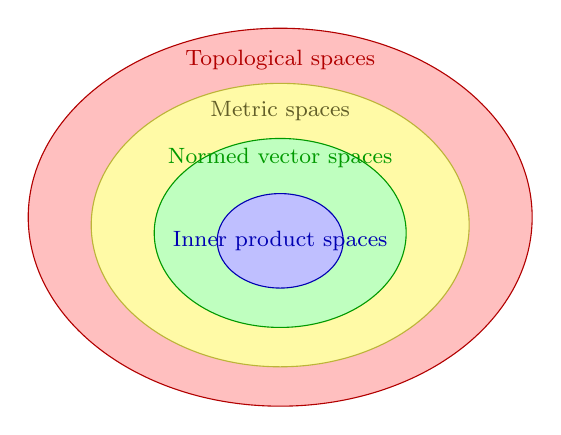
\begin{tikzpicture}
\fill[red!25] (0,0) ellipse (3.2 and 2.4);
\fill[yellow!35] (0,-0.1) ellipse (2.4 and 1.8);
\fill[green!25] (0,-0.2) ellipse (1.6 and 1.2);
\fill[blue!25] (0,-0.3) ellipse (0.8 and 0.6);
\draw[red!70!black] (0,0) ellipse (3.2 and 2.4);
\draw[yellow!70!black] (0,-0.1) ellipse (2.4 and 1.8);
\draw[green!60!black] (0,-0.2) ellipse (1.6 and 1.2);
\draw[blue!70!black] (0,-0.3) ellipse (0.8 and 0.6);
\node[red!70!black] at (0,2.0) {\footnotesize Topological spaces};
\node[olive!60!black] at (0,1.35) {\footnotesize Metric spaces};
\node[green!60!black] at (0,0.75) {\footnotesize Normed vector spaces};
\node[blue!70!black] at (0,-0.3) {\footnotesize Inner product spaces};
\end{tikzpicture}
\end{center}

You will see that an \textbf{inner product} $\langle\cdot,\cdot\rangle$ induces a \textbf{norm}
by the formula
\[\|x\| := \sqrt{\langle x, x\rangle}, \qquad x \in X.\]
Furthermore, a \textbf{norm} induces a \textbf{metric} by
\[d(x,y) := \|x - y\|, \qquad x, y \in X.\]

% Moved here from Week 3 (\S Cauchy--Schwarz): Corsin defines inner products and norms on the
% Friday of Week 3, but the two supplements below -- and the two displayed formulas above --
% already use both, so the definitions are stated here, at the point of first use. Corsin's own
% development of the geometry (angle, projection, the second proof of Cauchy--Schwarz) stays
% where he taught it, in \cref{sec:cauchy_schwarz}.
\begin{definition}[Inner product / scalar product]
\label{def:inner_product}
Let $V$ be a \textbf{vector space} over $\mathbb{R}$. An \newterm{inner product}
\germanfor{Skalarprodukt} on $V$ is a map
\[
\langle\cdot,\cdot\rangle : V \times V \to \mathbb{R}
\]
satisfying, for all $u, v, w \in V$ and $\alpha, \beta \in \mathbb{R}$:
\begin{enumerate}[label=\textbf{(\alph*)}]
  \item \textbf{Bilinearity:}
    $\langle \alpha u + \beta v, w\rangle = \alpha\langle u,w\rangle + \beta\langle v,w\rangle$,
    and equivalently in the second variable.
  \item \textbf{Symmetry:} $\langle u,v\rangle = \langle v,u\rangle$.
  \item \textbf{Definiteness:} $\langle u,u\rangle \geq 0$, and $\langle u,u\rangle = 0 \iff u = 0$.
\end{enumerate}
\end{definition}

\begin{definition}[Norm]
\label{def:norm}
Let $V$ be a \textbf{real} vector space. A \newterm{norm} \germanfor{Norm} on $V$ is a map
$\|\cdot\| : V \to [0,\infty)$ satisfying, for all $u, v \in V$ and $\alpha \in \mathbb{R}$:
\begin{enumerate}[label=\textbf{(\alph*)}]
  \item \textbf{Definiteness:} $\|v\| \geq 0$, and $\|v\| = 0 \iff v = 0$.
  \item \textbf{Homogeneity:} $\|\alpha v\| = |\alpha|\|v\|$.
  \item \textbf{$\Delta$-inequality:} $\|u+v\| \leq \|u\| + \|v\|$.
\end{enumerate}
\end{definition}

% Supplement: Analysis_II_Script_v1.pdf, p. 31
\begin{ainote}
The official script (Remark 9.94, p.\ 31 onward) adopts the opposite notational convention from
this document: from that point on \emph{it} writes the Euclidean norm as $|x|$ and reserves
$\|\cdot\|$ for non-standard norms. This document instead uses $\|\cdot\|$
(\texttt{\textbackslash lVert}\ldots\texttt{\textbackslash rVert}) uniformly for every norm,
Euclidean or not, per the house style, and keeps that convention throughout. Neither choice is
more standard than the other; this note exists only to warn anyone cross-referencing the script
directly that a bare $|\cdot|$ there and a bare $\|\cdot\|$ here can both denote \qt{the}
Euclidean norm. The warning matters most in the script's chapters 13--14, where the $|\cdot|$
convention is used densely.
\end{ainote}

% Source: Jérôme Paschoud/Notizen/Woche 4.1 Normen, das Differential.pdf, p. 1
% Generator: Gemini 3.1 Pro (High)
\begin{example}[Hilbert--Schmidt norm on matrix spaces]
\label{ex:hilbert_schmidt_norm}
A very important example of a norm on the space of real $n \times m$ matrices
$\mathbb{R}^{n \times m}$ is the \newterm{Hilbert--Schmidt norm} (also known as the Frobenius
norm). It is defined by
\[
\|M\|_2 := \sqrt{\Tr(M\transp M)},
\]
where $\Tr$ denotes the trace of a matrix. Only the diagonal of $M\transp M$ is needed, so the
off-diagonal entries are left unevaluated below. For a $2 \times 3$ matrix
$M = \left(\begin{smallmatrix} a & b & c \\ d & e & f \end{smallmatrix}\right)$, we have
\begin{align*}
M\transp M
  &= \begin{pmatrix} a & d \\ b & e \\ c & f \end{pmatrix}
     \begin{pmatrix} a & b & c \\ d & e & f \end{pmatrix} \\[0.6ex]
  &= \begin{pmatrix} a^2+d^2 & * & * \\ * & b^2+e^2 & * \\ * & * & c^2+f^2 \end{pmatrix}.
\end{align*}
The trace is the sum of the diagonal entries, so $\|M\|_2 = \sqrt{a^2+b^2+c^2+d^2+e^2+f^2}$. This
norm is therefore nothing but the standard Euclidean norm of the matrix entries read as a single
vector in $\mathbb{R}^{6}$, or in general in $\mathbb{R}^{nm}$. The inner product inducing it is
$\langle A, B \rangle := \Tr(A\transp B)$.
\end{example}

% Transition: Claude Opus 5 (High)
Comparing the three lists of axioms is already informative. A norm has exactly the three
properties a metric has, restated for a single vector instead of a pair of points, plus
homogeneity. That extra axiom has no metric analogue at all, since stating it requires scalar
multiplication. An inner product goes further and replaces the triangle inequality by
bilinearity, which is far stronger, and then recovers the triangle inequality as a \emph{theorem}
(\cref{prop:induced_norm_and_metric}) rather than assuming it. That is the precise sense in which
each layer carries more structure than the one outside it.

% The two blocks that follow supplement Corsin's outline with material from other tutors. They
% belong here logically, being about the innermost layer of the hierarchy just drawn, even though
% Corsin himself develops inner-product geometry only later (sec:cauchy_schwarz), where his own
% proof is kept. That prop:cauchy_schwarz_geometric_proof and thm:cauchy_schwarz are the same
% computation twice over is a mathematical point, and is made where it belongs, in
% rem:two_proofs_cauchy_schwarz.

% Supplement: Sascha Brack/Class Notes/Week_02_Notes_Monday_Updated.pdf, p. 4
\begin{remark}[Geometric angle and projection in inner product spaces]
\label{rem:inner_product_angle_geometry}
In an inner product space $(X, \langle\cdot,\cdot\rangle)$ over $\mathbb{R}$, the Cauchy--Schwarz inequality $|\langle x, y\rangle| \leq \|x\|\,\|y\|$ guarantees that for any non-zero vectors $x, y \in X$,
\[
-1 \leq \frac{\langle x, y\rangle}{\|x\|\,\|y\|} \leq 1.
\]
This allows us to formally define the \newterm{angle} $\Theta(x,y) \in [0,\pi]$ between $x$ and $y$ via
\[
\Theta(x,y) := \arccos\left(\frac{\langle x, y\rangle}{\|x\|\,\|y\|}\right).
\]
Geometrically, when $\|x\| = \|y\| = 1$, the inner product $\langle x, y\rangle$ is the signed
length of the orthogonal projection of $y$ onto the direction of $x$. In that reading
Cauchy--Schwarz becomes visually obvious: a projection of a unit vector cannot be longer than the
unit vector itself, so $\langle x,y\rangle \leq 1$, with equality exactly when $y$ already points
along $x$.
\begin{center}
% Generator: Claude Opus 5 (High) --- redrawn. The previous version parked a 6cm text block
% inside the picture, which pushed the figure off-centre and stated in words what the drawing
% should state by itself. Both vectors are unit, so they sit on the dashed unit circle; the
% angle arc now shows Theta, and the projection foot P = (cos 50, 0) is marked with a right
% angle. Angle 50 degrees: cos(50) = 0.643, sin(50) = 0.766.
\begin{tikzpicture}[>=Latex, scale=2.7]
  \coordinate (O) at (0,0);
  \coordinate (X) at (1,0);
  \coordinate (Y) at ({cos(50)},{sin(50)});
  \coordinate (P) at ({cos(50)},0);

  \draw[->, gray!55] (-0.18,0) -- (1.32,0);
  \draw[->, gray!55] (0,-0.18) -- (0,1.12);

  % both vectors are unit, so they end on this circle
  \draw[gray!40, dashed] (O) circle (1);

  % angle between x and y
  \draw[green!45!black, thick] (0.32,0) arc (0:50:0.32);
  \node[green!45!black, font=\footnotesize] at (0.50,0.17) {$\Theta$};

  % dropped perpendicular, with a right-angle mark at the foot
  \draw[blue!55, dashed] (Y) -- (P);
  \draw[blue!55] ({cos(50)-0.07},0) -- ({cos(50)-0.07},0.07) -- ({cos(50)},0.07);

  % The projection has to be measured BELOW the axis: drawn on the axis it would be collinear
  % with the arrow for x and simply disappear underneath it.
  \draw[orange!90!black, dotted] (0,0) -- (0,-0.17);
  \draw[orange!90!black, dotted] ({cos(50)},0) -- ({cos(50)},-0.17);
  \draw[orange!90!black, line width=0.9pt, <->] (0,-0.17) -- ({cos(50)},-0.17);
  \node[orange!90!black, font=\footnotesize, below] at ({cos(50)/2},-0.18)
    {$\langle x,y\rangle$};

  \draw[blue!60!black, thick, ->] (O) -- (X) node[above right, font=\small] {$x$};
  \draw[blue!60!black, thick, ->] (O) -- (Y) node[above left, font=\small] {$y$};

  \node[gray!55!black, font=\footnotesize, anchor=west] at (1.0,0.92) {$\|x\|=\|y\|=1$};
\end{tikzpicture}
\end{center}
\end{remark}

% Quelle: Diego Torres Tejeda/Notes - 09.03 - Diego Torres Tejeda.pdf, pp. 1--2
\begin{proposition}[Geometric derivation of the Cauchy--Schwarz inequality]
\label{prop:cauchy_schwarz_geometric_proof}
Let $(V, \langle\cdot,\cdot\rangle)$ be a real inner product space. Then for all $v, w \in V$,
\[
|\langle v, w\rangle| \leq \|v\|\,\|w\|.
\]
\end{proposition}

\begin{proof}
If $w = 0$, both sides vanish and the inequality holds trivially. For $w \neq 0$, consider the squared distance from $v$ to the points of the line $L := \operatorname{span}_{\mathbb{R}}\{w\}$, parametrized by $\lambda \mapsto \lambda w$:
\[
f(\lambda) := \|v - \lambda w\|^2 = \langle v - \lambda w, v - \lambda w\rangle = \|v\|^2 - 2\lambda\langle v, w\rangle + \lambda^2\|w\|^2.
\]
Since $f(\lambda) \geq 0$ for all $\lambda \in \mathbb{R}$, $f$ is a convex quadratic polynomial in $\lambda$ with positive leading coefficient $\|w\|^2 > 0$. Differentiating or completing the square shows that $f$ attains its global minimum at $\lambda_0 := \frac{\langle v, w\rangle}{\|w\|^2}$. Evaluating $f$ at $\lambda_0$ yields
\[
0 \leq f(\lambda_0) = \|v\|^2 - 2\frac{\langle v, w\rangle^2}{\|w\|^2} + \frac{\langle v, w\rangle^2}{\|w\|^2} = \|v\|^2 - \frac{\langle v, w\rangle^2}{\|w\|^2}.
\]
Multiplying by $\|w\|^2$ and taking square roots gives $|\langle v, w\rangle| \leq \|v\|\,\|w\|$. Geometrically, $\pi_L(v) := \lambda_0 w = \frac{\langle v, w\rangle}{\|w\|^2}w$ is the unique orthogonal projection of $v$ onto the line $L$, achieving the minimal distance $d(v, L) = \sqrt{f(\lambda_0)}$.
\end{proof}

% Generator: Claude Opus 5 (High) --- moved here from Week 3 together with \cref{def:norm}:
% Cauchy--Schwarz is now available (immediately above), which is the only input the triangle
% inequality needs, so the two arrows of the hierarchy can be justified where they are drawn.
\begin{proposition}[Inner product $\Rightarrow$ norm $\Rightarrow$ metric]
\label{prop:induced_norm_and_metric}
Let $V$ be a real vector space.
\begin{enumerate}[label=\textbf{(\alph*)}]
  \item If $\langle\cdot,\cdot\rangle$ is an inner product on $V$ (\cref{def:inner_product}),
    then $\|v\| := \sqrt{\langle v,v\rangle}$ is a norm on $V$ (\cref{def:norm}).
  \item If $\|\cdot\|$ is a norm on $V$, then $d(x,y) := \|x-y\|$ is a metric on $V$
    (\cref{def:metric_space}).
\end{enumerate}
\end{proposition}

\begin{proof}
\textbf{(a)} Definiteness of the norm is definiteness of the inner product, and homogeneity
follows from bilinearity: $\|\alpha v\|^2 = \langle\alpha v,\alpha v\rangle =
\alpha^2\|v\|^2$. For the triangle inequality, expand and apply
\cref{prop:cauchy_schwarz_geometric_proof}:
\begin{align*}
  \|u+v\|^2 &= \|u\|^2 + 2\langle u,v\rangle + \|v\|^2 \\
            &\leq \|u\|^2 + 2\lvert\langle u,v\rangle\rvert + \|v\|^2 \\
            &\leq \|u\|^2 + 2\|u\|\,\|v\| + \|v\|^2 \ =\ \big(\|u\|+\|v\|\big)^2,
\end{align*}
and taking square roots gives $\|u+v\| \leq \|u\|+\|v\|$.

\textbf{(b)} Definiteness: $d(x,y)=0$ means $\|x-y\|=0$, hence $x=y$. Symmetry: homogeneity
with $\alpha=-1$ gives $\|x-y\| = \|-(y-x)\| = \|y-x\|$. Triangle inequality: writing
$x-z = (x-y)+(y-z)$,
\[d(x,z) = \|(x-y)+(y-z)\| \leq \|x-y\| + \|y-z\| = d(x,y)+d(y,z). \qedhere\]
\end{proof}

\begin{remark}[Neither arrow reverses]
\label{rem:norm_not_from_inner_product}
The nesting drawn above is strict at both steps.
\begin{itemize}
  \item \textbf{Not every metric comes from a norm.} The discrete metric
    (\cref{ex:metric_examples}\textbf{(a)}) on a vector space cannot: a norm-induced metric
    satisfies $d(\alpha x, 0) = |\alpha|\,d(x,0)$, which fails as soon as
    $\alpha \neq 0,\pm1$.
  \item \textbf{Not every norm comes from an inner product.} A norm induced by an inner product
    obeys the \newterm{parallelogram law}
    $\|u+v\|^2 + \|u-v\|^2 = 2\|u\|^2 + 2\|v\|^2$ (expand both sides by bilinearity). The
    supremum norm on $\mathbb{R}^2$ violates it: for $u := (1,0)$ and $v := (0,1)$ the left side
    is $1+1 = 2$ and the right side is $2+2 = 4$.
\end{itemize}
Consequently, each layer of the hierarchy really does carry strictly more structure than the one
outside it. The picture at the start of this section is a genuine nesting of four distinct
classes, not a chain of equivalent descriptions of the same thing.
\end{remark}

% Source: Corsin Nick/Class Notes/Week 2.pdf, pp. 1--13
